% !TeX root = ../main.tex

\chapter*{主要布局要求V1.4}
\section*{原理图更新日志 2023.09.25}
\textcolor{red}{
  \begin{enumerate}
    \item PCB右侧的接口不要露出板框。
    \item J21、J23 两个接口的六个通孔排成一排,且与板框留出8mm的距离。
    \item 地测试孔与电源测试孔成对出现,J20连接器向左移动,J19 开关方向改为水平,放在J18上方(这里请看J19开关手册,把拨码露在板框外)。
    \item U27、U31为FPGA和ARM之间通信的芯片,放在二者中间,可适当增加FPGA 和 ARM 之间距离。
    \item 为方便布线,更新了 U28、U31所连接的ARM管脚位置。
    \item 除了PCB右侧的两种接口,其余接口均可根据布线方便进行调整,PCB左侧除了电源,尽量不要留有其他接口。
    \item 右侧两个接口器件摆在和SEAF所连接信号的不同侧,防止干扰。
  \end{enumerate}
}
\section*{原理图更新日志 2023.09.24}
\begin{enumerate}
  \item 为方便器件采购,更新了一些电容电阻封装。
\end{enumerate}
\section*{原理图更新日志 2023.09.22}
\begin{enumerate}
  \item 更新了LVDS接口及布局
  \item 删除了FPGA所连接的Ethernet接口(原理图GbE1页面)
\end{enumerate}

\bigskip
\begin{enumerate}
  \item 12 层板,mil 为单位
  \item 整板尺寸 \SI{10512}{mil} $\times$ \SI{6142}{mil},倒角 \SI{120}{mil}
  \item 安装孔相对板子中心坐标:$(-5020, 2835)$、$(-5020, -2835)$、$(2106, -2835)$、$(5020, -2835)$、$(5020, 2835)$、$(2106, 2835)$
  \item 该PCB正面(TOP层)与一块核心板 FET3568-C (外观图如图~\ref{fig:FET3568-COutlook}所示)通过四个连接器(原理图 FET3568J-C 页面:J10(左上)、J11(右上)、J12(左下)、J13(右下),分别对应核心板:P1、P2、P3、P4)相连,核心板尺寸图如图~\ref{fig:FET3568-CSize} 所示(单位: mm),更多详细尺寸请见:\verb|"Appendices/核心板 1.0 DXF 文件"|内的 dxf 结构文件。
  \begin{figure}
    \centering
    \begin{subfigure}{0.8\textwidth}
      \centering
      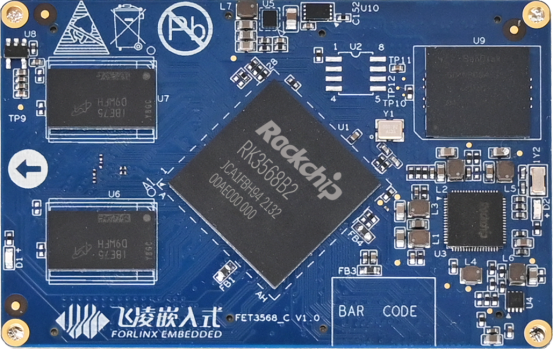
\includegraphics[width=\textwidth]{./figures/FET3568-C核心板外观图TOP.png}
      \caption{FET3568-C 核心板正面图}
      \label{fig:FET3568-COutlookTop}
    \end{subfigure}
    \begin{subfigure}{0.8\textwidth}
      \centering
      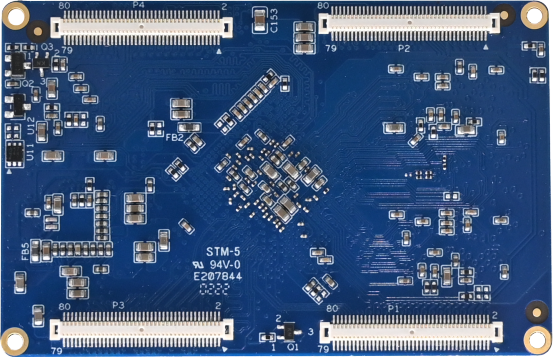
\includegraphics[width=\textwidth]{./figures/FET3568-C核心板外观图BOTTOM.png}
      \caption{FET3568-C 核心板背面图}
      \label{fig:FET3568-COutlookBottom}
    \end{subfigure}
    \caption{FET3568-C 核心板外观图}
    \label{fig:FET3568-COutlook}
  \end{figure}
  \begin{figure}
    \centering
    \begin{subfigure}[b]{0.8\textwidth}
      \centering
      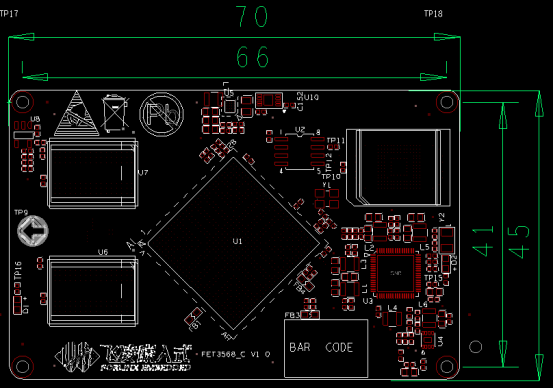
\includegraphics[width=\textwidth]{./figures/FET3568-C核心板尺寸图TOP.png}
      \caption{FET3568-C 核心板尺寸图TOP}
      \label{fig:FET3568-CSizeTop}
    \end{subfigure}
    \begin{subfigure}[b]{0.8\textwidth}
      \centering
      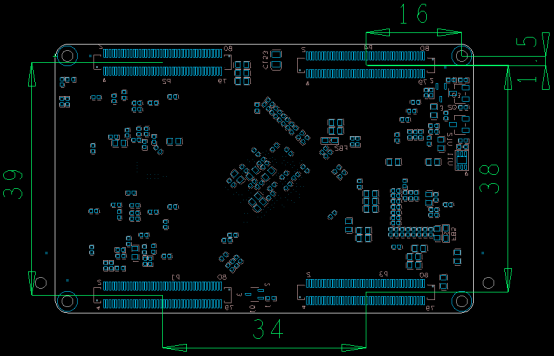
\includegraphics[width=\textwidth]{./figures/FET3568-C核心板尺寸图BOTTOM.png}
      \caption{FET3568-C 核心板尺寸图BOTTOM}
      \label{fig:FET3568-CSizeBottom}
    \end{subfigure}
    \caption{FET3568-C 核心板尺寸图}
    \label{fig:FET3568-CSize}
  \end{figure}

  \item 核心板的四角预留了四个直径 2.2mm 的安装孔,在该PCB中应使用 M2, L=2mm 的贴片螺母(M7、M8、M9、M10,未提供封装,\emph{需更换PCB Footprint}),贴片螺母的规格参见图~\ref{fig:M2Size}
  \begin{figure}
    \centering
    \begin{subfigure}[b]{0.35\textwidth}
      \centering
      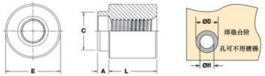
\includegraphics[width=\textwidth]{./figures/M2_fig.png}
    \end{subfigure}
    \begin{subfigure}[b]{0.7\textwidth}
      \centering
      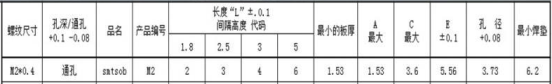
\includegraphics[width=\textwidth]{./figures/M2_tab.png}
    \end{subfigure}
    \caption{M2 贴片螺母尺寸}
    \label{fig:M2Size}
  \end{figure}

  \item 500 pin 高密连接器 SEAF 是模拟信号输入端,放在电路板背面(bottom 层),右侧正中心,
  \item 从 SEAF 到ADC包括130对差分对输入信号,该部分为模拟信号,附近请不要覆盖任何数字电源层,以干扰模拟信号质量。
  \item ADC(ADS52J90)输出到FPGA为JESD高速信号,请保证同ADC的不同输出信号线以及不同ADC的输出信号线(包括时钟)到FPGA的长度尽量等长,以保证时钟同步性。
  \item ADC(AD9635)输出到FPGA的信号为LVDS,请保证同ADC的不同输出信号线(包括时钟)到FPGA的长度尽量等长,以保证时钟同步性
  \item FPGA 与 核心板之间的 8 位GPIO信号做等长。
  \item USB3.0 设计规则
  \begin{itemize}
    \item USB3.0 端口设计采用点对点方式, U3\_TX\_DP、 U3\_TX\_DN 需要采用AC 耦合,耦合电容放在离终端近的位置。
    \item USB信号需要采用差分布线, 阻抗 \SI{90}{\upOmega} $\pm 10\%$。
    \item USB布线长度不超过\SI{150}{mm}, 差分对内信号长度误差不超过\SI{0.12}{mm}。
    \item ESD 器件离USB接口不超过\SI{12}{mm},共模扼流圈离USB接口不超过\SI{25}{mm}。
  \end{itemize}
  \item SDMMC0\_*设计规则
  \begin{itemize}
    \item SDMMC0 信号阻抗 \SI{50}{\upOmega} $\pm 10 \%$。
    \item SDMMC0 接口信号要做等长控制,误差不超过 \SI{0.25}{mm}。
    \item 布线尽量短,串联端接电阻应靠近输出端。
  \end{itemize}
  \item LVDS 信号需要采用差分布线, 阻抗 \SI{100}{\upOmega} $\pm 10\%$,各差分信号之间预留 \SI{100}{\upOmega} 电阻焊接位置。
  \item Ethernet 设计规则
  \begin{itemize}
    \item RGMII 接口分为发送信号, 接收信号和控制信号, 各组阻抗控制在 \SI{50}{\upOmega} $\pm 10\%$。
    \item 发送信号和接收信号,布线长度不超过 \SI{100}{mm},组内信号长度误差不超过 \SI{2.54}{mm}。
    \item MDI 接口采用差分布线, 阻抗 \SI{100}{\upOmega} $\pm 10\%$。组间等长要求 $\leq$ \SI{1000}{mil}
    \item MDI 组内差分误差不超过 \SI{0.12}{mm}。
    \item 芯片内部 DCDC 连接的功率电感要靠近芯片保证回路最短, 并且保证地回路的完整
    \item 数据线上预留的串联电阻需要靠近源端放置
    \item 保护器件建议放置在变压器内侧, 在变压器和 PHY 之间, 靠近变压器
  \end{itemize}
  \item FPGA 与 核心板之间的 PCIe 设计规则
  \begin{itemize}
    \item PCIe 信号设计采用点对点方式,耦合方式采用AC耦合,耦合电容放在离发送端近的位置。
    \item PCIe收发数据信号需要采用差分布线, 阻抗\SI{85}{\upOmega}$\pm 15\%$。
    \item PCIe时钟信号采用差分布线, 阻抗 \SI{100}{\upOmega} $\pm 10\%$。
    \item 差分对总长度不超过 \SI{300}{mm}, 差分对内长度误差不超过 \SI{0.12}{mm},同方向的差分对间长度误差不超过 \SI{180}{mm}, 差分对间距离不低于\SI{0.3}{mm}。
  \end{itemize}
  \item 原理图 \emph{LVDS\_FPGA} 页面的芯片及接口放在电路板右侧,该接口为数字信号传输端,应保证该页面信号远离高密连接器 SEAF 及其所连接的模拟信号。
  \item 原理图 \emph{RS485\_External} 页面的芯片及接口放在电路板右侧(不伸出板框),该接口为数字信号传输端,应保证该页面信号远离高密连接器 SEAF 及其所连接的模拟信号
  \item 原理图 \emph{USB3.0} 页面的接口(MOLEX\_2171790001、MOLEX\_0484050003),其中 MOLEX\_0484050003 放电路板正面,MOLEX\_2171790001 放在电路板背面(MOLEX\_0484050003 正下方)
  \item 除 \emph{LVDS\_FPGA}和 \emph{RS485\_External} 之外的接口可根据布局进行调整,数据流向为从右到左(SEAF $\rightarrow$ ADC $\rightarrow$ FPGA $\rightarrow$ ARM 核心板)。
  \item 线距满足3W原则,线宽普通走线\SI{8}{mil},电源和地走线不小于\SI{20}{mil}。命名为$\pm$或pn、pm的为差分对,线长差原则上在\SIrange{20}{50}{mil}之间,线宽\SI{6}{mil},线距\SI{12}{mil}(线中心到线中心)。标注A的模拟电源层与标注D的数字电源层分开。
  \item 更进一步的细节和布局改动可继续讨论。请尽快确认布局,若有无法满足的情况请尽早沟通。
\end{enumerate}